The methods we will discuss in this thesis are ultimately about improving the performance of software. 
We need benchmarks to assess the performance of software and its improvements.
Benchmarks are essential for the research and development of compilers and programming languages~\cite{hall_compiler_research}, as well as hardware architectures or runtime systems.
In this context, benchmarks are generally understood to be collections of programs with particular properties.
Mostly, they cover a range of behaviors that are typical of, and important for programs in a particular domain.
This description, however, can mean several different things.
% In this section, we formally define different classes of benchmarks and argue how they might be desirable in different scenarios.
In this chapter, we formally define different types of benchmarks and use them to classify different use cases.
We then proceed to discuss concrete \ac{KPN} and task-graph benchmarks for software synthesis, as well as benchmark generation strategies both with random graph models and machine learning.


\begin{figure}[t]
	\centering
	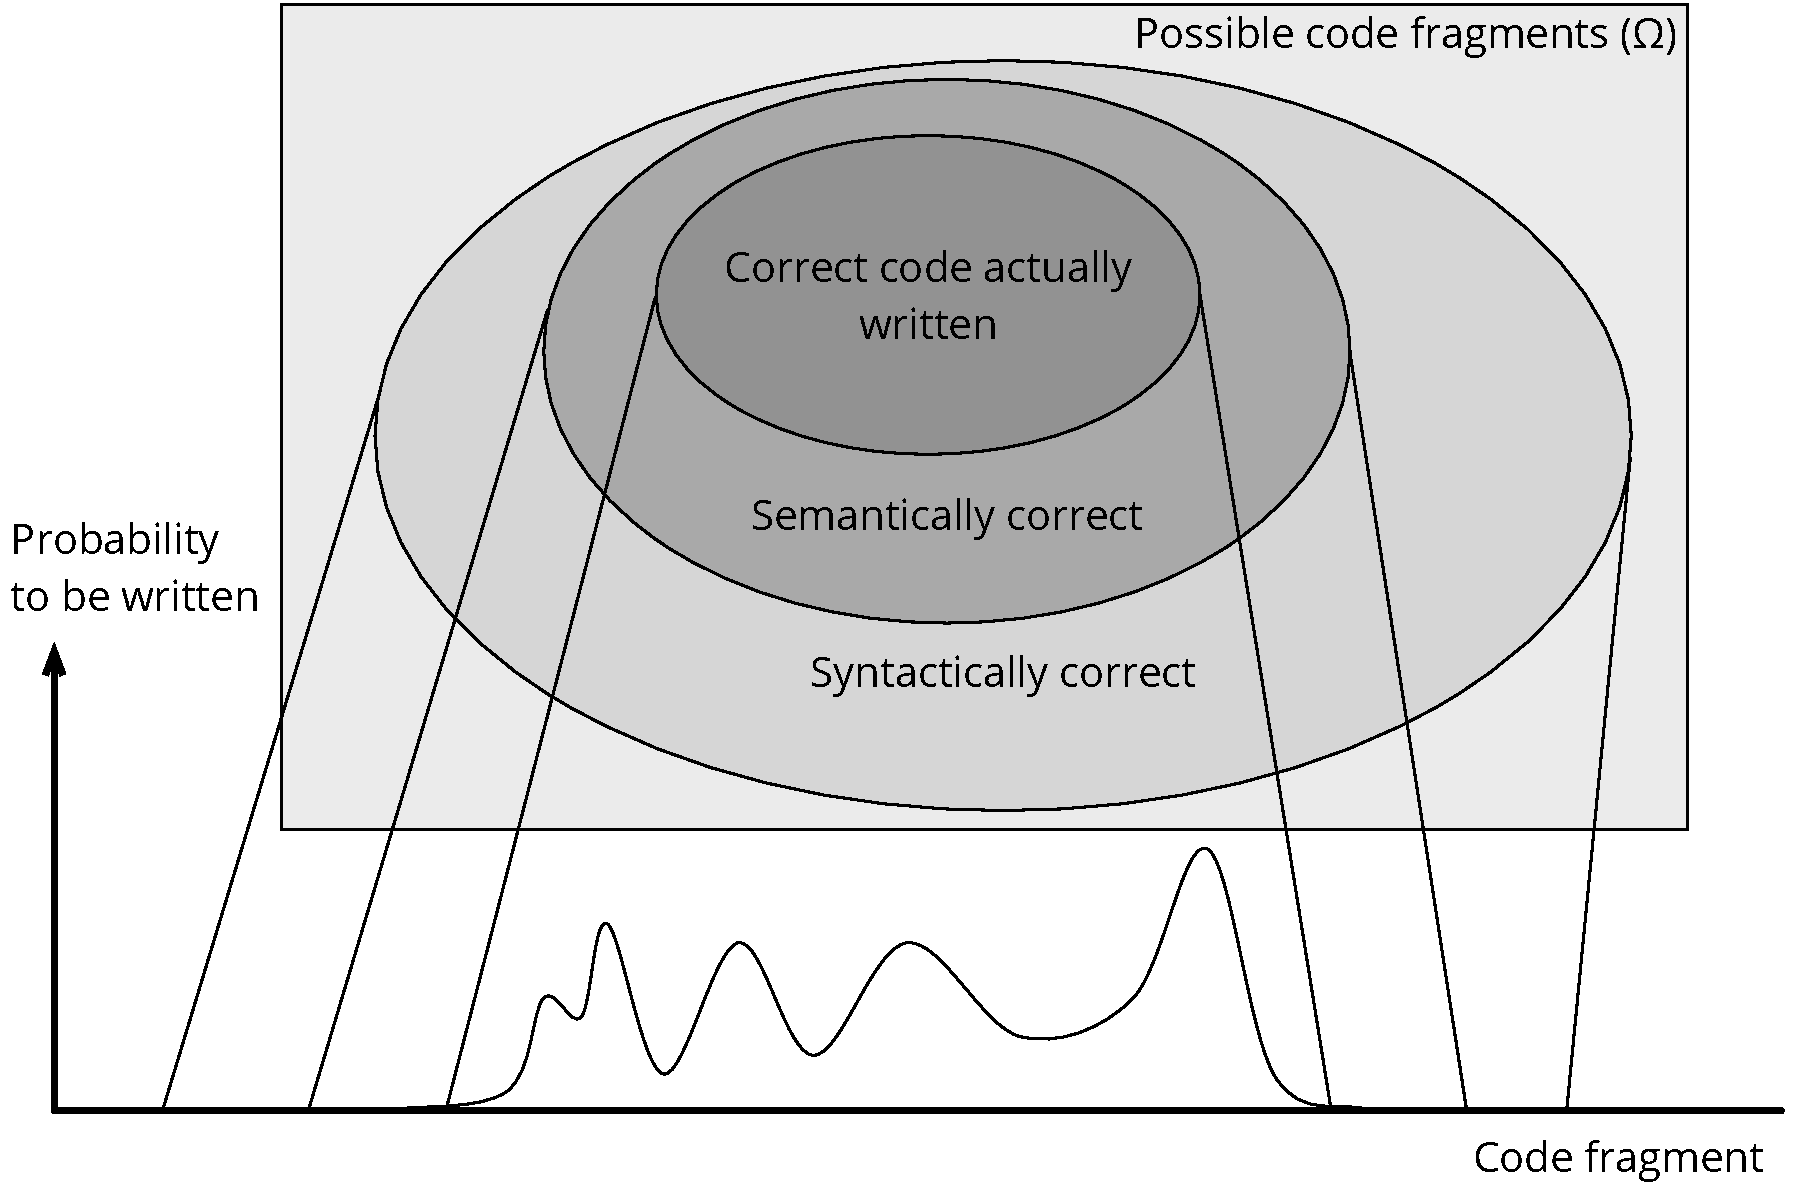
\includegraphics[width=0.4\textwidth]{figures/code_space_venn.pdf}
	\caption{An illustration of probabilities in code space}
	\label{fig:pdf_programs}
\end{figure}


To formalize our argumentation, we take a statistical view of program code.
Consider the formal language that describes the set of all possible programs.
For a program of fixed bounded size, this is a finite set $\Omega$.
For example, the set of syntactically correct C source files smaller than $10$~TiB in size is certainly bounded by $|\Omega| = 10 \cdot 2^{40}$.
% For example, a source file $\omega \in \Omega$  under $10$ tebibyte (TiB), syntactically correct ones are certainly bounded by $|\Omega| = 10 \cdot 2^{40}$, probably a much lower number.
Out of the syntactically-correct programs, only a fraction successfully compiles, and only an even smaller fraction executes something that makes sense semantically.
Ideally, code written by developers falls into the subset of executable programs, as an even smaller subset.
However, in this subset of correctly written code, not every code fragment is going to be equally common.
A fragment like
\texttt{for(int i = 0; i < n; i++)} is probably going to be seen much more frequently than something like \texttt{(*(\&main+0x134))(x)}.
It is worth noting that there is a more nuanced discussion behind what constitutes a unit of code.
At this point, however, we can omit this discussion and consider the whole program as a unit, for simplicity of the argumentation.
%\se{Do we lose generality of our argument because of this? If not then we should say so.} % AG: I don't think we do, no.
Thus, there is an implicit \ac{pdf} $p$ on the discrete set of possible code units $\Omega$ which models the way programmers write code.
This is depicted in Figure~\ref{fig:pdf_programs}.
In reality, this is a highly dimensional space, and many challenges would arise in defining a proper geometry in such a space.
We depict the code space $\Omega$ as one-dimensional for illustrative purposes, just like the continuity of the \ac{pdf}, which we have no reason to assume.

\subsection{Representative Benchmarks}
\label{sec:representative_benchmarks}

\begin{figure}[th]
	\centering
	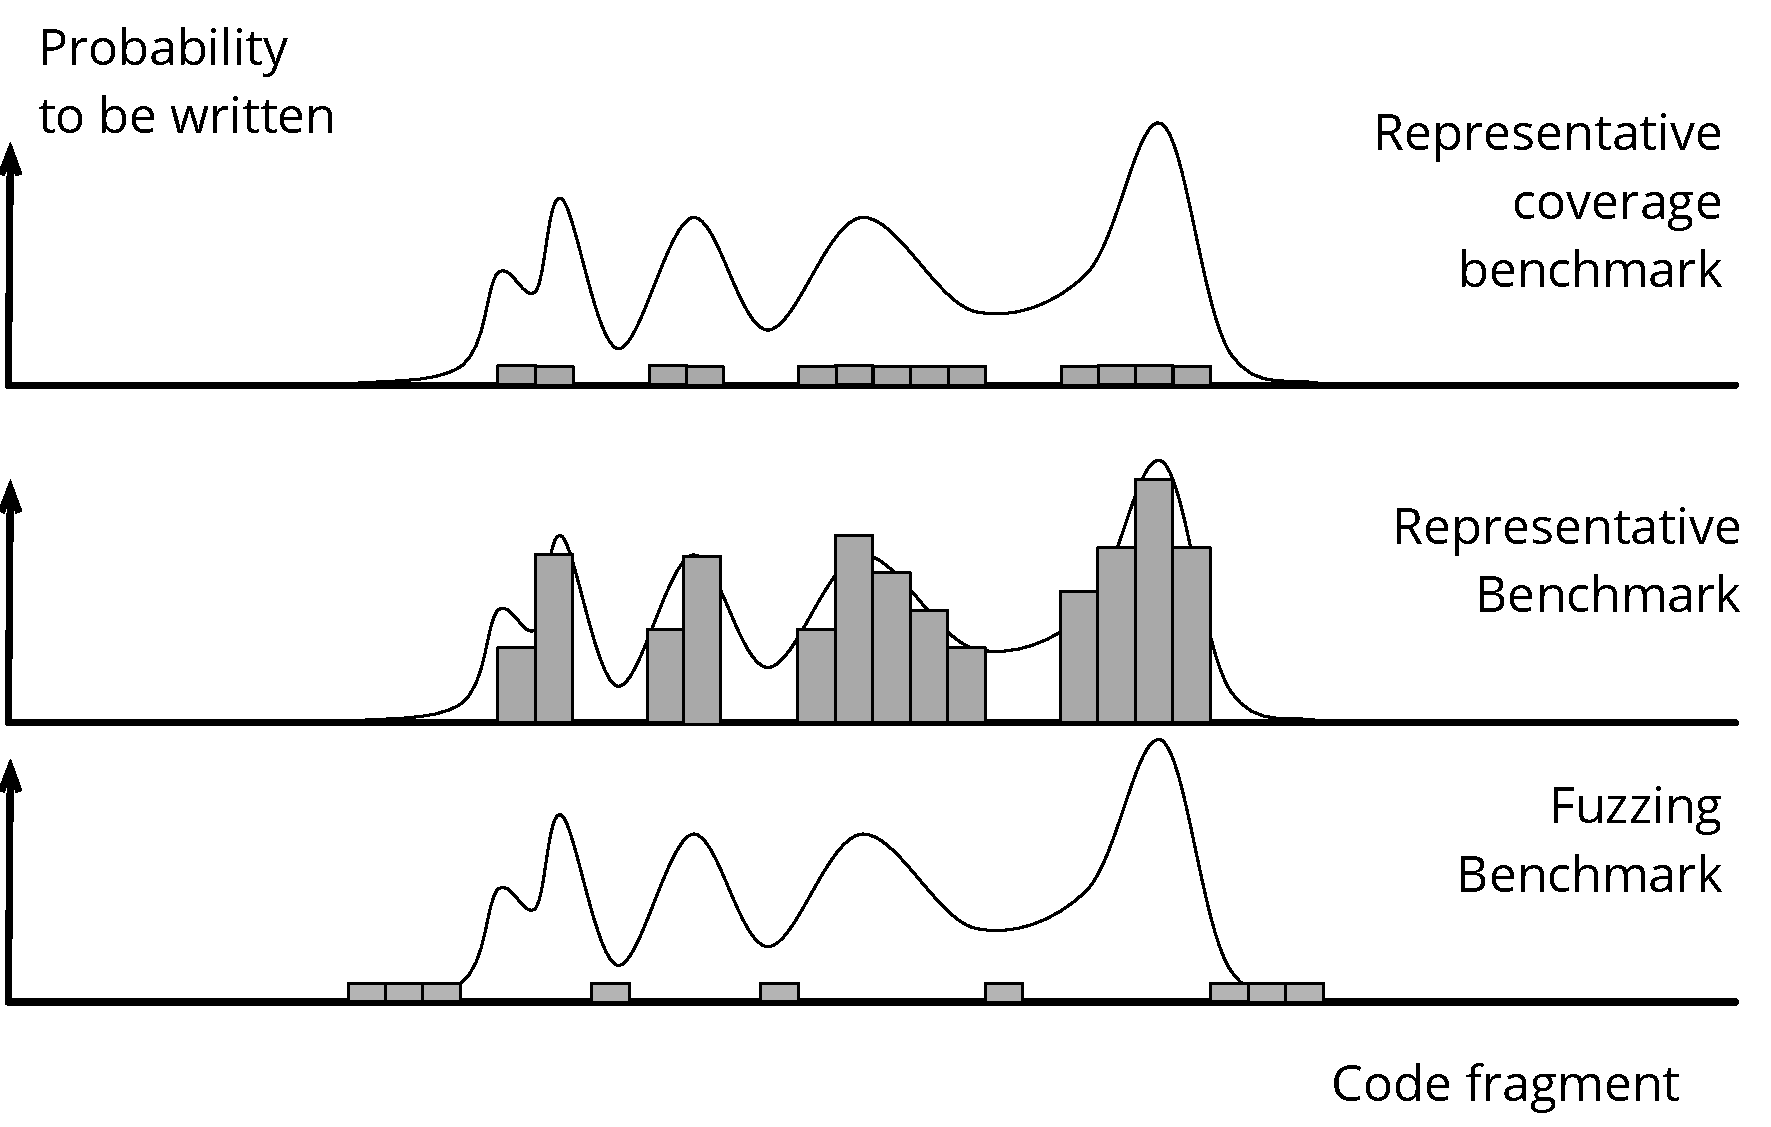
\includegraphics[width=0.5\textwidth]{figures/benchmark_types.pdf}
	\caption{An illustration of different types of benchmarks}
	\label{fig:benchmark_types}
\end{figure}

In this statistical view of code, we can consider some precise questions: What does it mean for a collection of programs to be a benchmark?
More precisely, what does it mean for it to be representative, or what properties would be desirable of such a collection of programs?
Consider the examples depicted in Figure~\ref{fig:benchmark_types}.
This figure depicts histograms for three kinds of collections of programs along the (implicit) pdf described in Figure~\ref{fig:pdf_programs}.
We think of an idealized abscissa dimension, with a proper metric, such that programs that are semantically close are close on this dimension.
Obviously a multi-dimensional formalization would be better for this, but we stick to a single dimension for the intuition provided by the figures.
Thus, a bin in the histogram might contain a single program but represent a large category of mostly very closely related programs.

The first kind of collection depicted, labeled as a ``representative coverage benchmark'', has a handful of programs, each of which corresponding to a different category in the space of probable programs.
Programs that could be written by a human, but where it is unlikely that this will happen, are not covered by this type of benchmark. Furthermore, for every type or category of code fragments, there is only one representative example in the set.
In particular, programs that are moderately likely will be represented just as much as programs that are extremely likely to be written. This, in a sense, overrepresents the former and underrepresents the latter.

The second kind depicted, labeled as ``representative benchmark'', removes this imbalance. It is similar to the ``representative coverage benchmark'', but the difference is that in this kind of collection, programs appear with a relative frequency that is roughly in line with their probability to be written.
A benchmark of this kind would probably have more programs than a ``representative coverage benchmark'', without including significantly more types of programs or behaviors.

Finally, a ``fuzzing benchmark'' is a collection that does the opposite of a ``representative coverage benchmark''. It has programs covering those programs that are unlikely to be written by a human, but possible: The corner cases.

%This pdf is what a generative model can learn.
%More formally, consider the generative model of code learning from these samples.
%Generative models are a class of machine learning problems that learn an unknown probability distribution for a random variable~\cite{vapnik}.
\subsection{Sample use cases}

We argue that what kind of benchmark is most appropriate depends on the use case. To illustrate this, we will explain two large classes of use-cases that require benchmarks. This certainly does not constitute an exhaustive classification, but will hopefully help clarify how the benchmark choice is nuanced.

\subsubsection{Testing}
\label{sec:testing}

A very common use case for benchmarking is testing. Assume we have developed a compiler optimization and want to see how good it works.
For this, we want to find out, in case someone writes a program and tries our optimization on it, how we can expect it to behave.
More formally, we have a property $\mathcal{P}$ of code, like the speedup obtained by applying our compiler optimization.
We want to calculate the expected value $E[\mathcal{P}]$ over the implicit pdf of writing the code we use our compiler on\footnote{Technically, using the compiler is a conditional clause on the probability of a piece of code to be written by a human. See Section~\ref{sec:outlook} for a discussion of this.}.

For testing, we argue that we want a \emph{representative} benchmark. Ideally, we would get a set of programs $x_1, \ldots, x_l \sim p$ i.i.d., where $p$ is the implicit probability density function of code been written\footnote{A compelling case can be made that in some cases it's the ``dynamic'' property of the probability that a piece of code will be \emph{executed}, not necessarily written, that is most interesting here.}.
The expected value $E[\mathcal{P}]$ can thus be approximated arbitrarily well with growing sample size $l$.
We do this because, in our example, we assume that the users of our compiler will also draw from this distribution $p$, and thus $E[\text{speedup}]$ tells us what speedup the users can expect to get out of our optimization.

If we use a ``representative coverage benchmark'', we can get a skewed result, because of the over- and underrepresentation of program types in this kind of benchmark.
Thus, if our optimization works extremely well for a small class of programs with a moderate chance of occurring, and not so well with the most common types of programs, our testing would return wrong results.
It would tell us that our optimization is likeley to improve our program, by overshooting the weight given to the moderately common class where it serves well.
In practice, however, our optimization would be unlikeley to bring much improvement in this case, if we expect our compiler to be used by everyone.

\subsubsection{Tuning a Heuristic}
\label{sec:tuning}

Another common use case is tuning a heuristic. Consider again a compiler optimization as an example. In this case, however, instead of having a finished optimization that we want to test, we are designing the optimization by tuning a heuristic that is part of it.
We want the heuristic to be tuned such that the optimization works best (which we would asses e.g. by testing, the other use-case).
Training machine learning models also falls under this category, and is thus likely that this use case will continue to increase in its importance in the feature.

For tuning the heuristic, an argument can be made for all three kinds of benchmarks from Figure~\ref{fig:benchmark_types}. It depends on the heuristic.
Assume we're dealing with a code transformation (e.g. converting Python 2 code automatically into Python 3),  which either it works or it doesn't. We want to optimize the parameters of our heuristic so that it works on the most cases possible.
In this case we probably want a ``fuzzing benchmark'', to be sure we cover the corner cases, or better yet, a combination of a ``fuzzing benchmark'' and a ``representative coverage benchmark''.
On the other hand, if the heuristic is something like a transformation expected to speed up the execution, then the argument for a ``representative benchmark'' is basically the same as for testing.
We want it maximize the expected value of this speedup.
An important distinction between heuristics pertains the way the parameters are set. Depending on how they are updated, repeatedly seeing similar code examples might be useless or even counter-productive, such that a ``representative coverage benchmark'' might be best suited.

More importantly yet is the process of designing the heuristic, before it is tuned. Usually this process is iterative. In it, having to look at the corner cases is common, too.
Arguments for all the discussed kinds of benchmarks can thus be made in similar fashion for the process of designing a heuristic, depending on specific goals.

